\chapter{System Design}

\section{Business case}

ChatX is a chatting system which will allow users to communicate with each other from where ever they are and without fear of the messages being read by unwanted users, as long as they use a platform that supports the application and have a internet connection.

\subsection{What issue will ChatX solve?}
It will be possible to integrate the system with other systems where users could have need of communication with other users on a secure connection that will be hard for others to sniff data from. Thus making sure that messages are private and only seen by the intended users.

\subsection{FURPS}

\subsubsection{Functionality}

\subsubsection{Usability}

\subsubsection{Reliability}

\subsubsection{Performance}

\subsubsection{Supportability}

\section{Architecture}
ChatX's architecture will be a client-server architecture. The client will call the server whenever a user requests to use the system and the server will keep track of how many users are online and where each user messages is suppose to be sent to.

\subsection{Domain Model}

\begin{figure}[H]
\centering
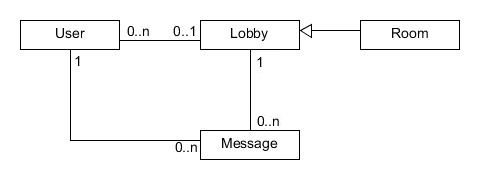
\includegraphics[width=0.7\linewidth]{img/DomainModelChatX}
\caption{Domain Model over ChatX}
\label{fig:DomainModelChatX}
\end{figure}

The domain model consists of four classes. The user class is where users are identified and if they are regular users or administrative users, a user can only be in one lobby at a time but a lobby can have multiple users. A user can also none to many messages. The message class is used for sending messages between users, a user can have none to many messages, whilst a message can only belong to one user. The lobby is where all users start. From the lobby a user can create a room and choose which users are to be included in it, the room class inherits the functionality of the lobby class.
